\section{Relations Groupes/Sessions}

Maintenant que nous avons exploré les concepts de groupes de processus et de sessions, l'exemple en shell ci-dessus offre une opportunité pratique d'illustrer comment ces notions interagissent dans un environnement Unix/Linux.

\begin{lstlisting}[language=sh,basicstyle=\small]
$ echo $$ # PID du shell
1001
$ ls /home | grep "user" & # 2 process dans le groupe background
[1] 1023
$ cat logs.txt | grep "sys5" # 2 process dans le groupe foreground
\end{lstlisting}

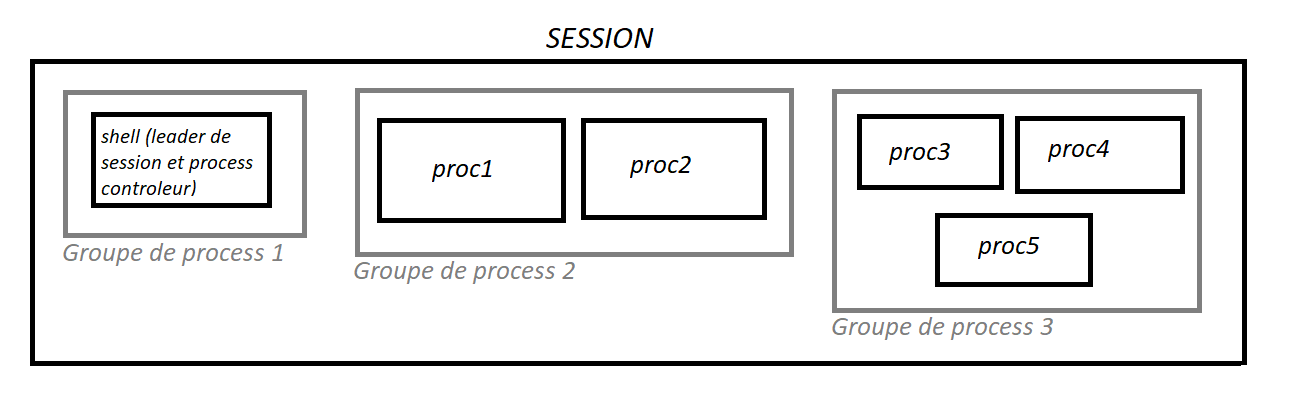
\includegraphics[width=1\textwidth]{img/SessionEtGroupes.png}